\section{Specific Requirements}

\subsection{External Interfaces}

\subsubsection{System Interfaces}

\paragraph{Municipality Data Exchange} \label{p:mde} The definition of the municipality data exchange interface is dependent to the corresponding SafeStreet's interface required to be offered to the municipalities. The municipality is required to offer the following functionalities to the system:

	\begin{itemize}
		\item Guarantee a secure authentication to the municipalities' system using a provided \emph{restricted access API}
		\item Provide a secure transfer of data related to accidents occurred in the territory of the municipality
		\item Provide a secure transfer of data related to local authorities' issued tickets 
	\end{itemize} 
	
	Leveraging the retrieved municipality data the system is required to cross this information with the system previously stored data. In addition, the system is required to perform the following functions on the crossed data:
	
	\begin{itemize}
		\item Build statistics on the frequency of violations
		\item Build statistics on the users that submit the most violations
		\item Build statistics on the cities with the highest number of violations
		\item Build statistics on the effectiveness of the SafeStreets initiative by looking for trends in the issuing of tickets
		\item Identify potentially unsafe areas and store this new generated information 
		\item Identify possible interventions to be suggested to the municipalities and store this new generated information 
	\end{itemize}
		
	To fulfil the bidirectional data exchange the system is required to offer the following functionalities to the municipalities:
	
	\begin{itemize}
		\item Guarantee a secure authentication to the system using a provided \emph{restricted access API}
		\item Provide a secure transfer of data related to user uploaded violations and all the corresponding metadata
		\item Provide a secure transfer of data related to possible interventions suggestions 
		
	\end{itemize} 
	
\clearpage

\paragraph{Geographic Information System} \label{p:gis} The definition of the external GIS interface is GIS dependant and will be described in a functionality-based way. The system is required to perform the following functions:

	\begin{itemize}
		\item Load and filter data based on the user requested criteria
		\item Cache retrieved data for the most common user requested criteria
		\item Communicate the loaded and filtered data to the external GIS with the final goal of presenting the requested map to the user via the user interfaces
		
		\end{itemize}
	
	The system via the external GIS is required to be capable of handling the following data visualisations:
	
	\begin{itemize}
		\item Visualise the spatial location of stored violations inside a specific geographic area requested by the user
		\item Visualise the spatial location of stored violations inside a specific geographic area and a specific time range requested by the user
		\item Visualise the distinction between possible safe and unsafe areas identified by the system
		\item Map quantities and concentrations, such as where the most and least number of violations occurred, highlighting the streets (and areas) with the highest frequency of violations
		\item Map the change of quantities and concentrations inside a specific geographic area and a specific time range requested by the user \newline
	\end{itemize}

	\begin{figure}[h]
		\centering
		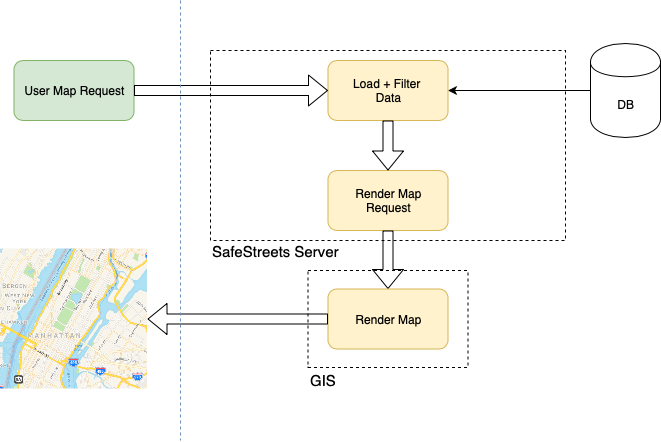
\includegraphics[width=335pt]{diagrams/GIS.png}
		\caption{
			\label{fig:externalGIS} GIS Interaction Diagram}
	\end{figure}

\subsubsection{User Interfaces}

	One of the key methodologies to capture the goals that the system's user interfaces must satisfy is through user interfaces mockups. The same structure of the overall description \hyperref[sec:goals]{corresponding section} will be used in order to extend the already stated requirements.

 \paragraph{Guest User}

	\begin{itemize}
		\item The system is required to offer guest users the ability to register to the system. The personal ID and a valid e-mail address are required for the registration in order to verify the authenticity of the new account. A password policy, composed of a set of rules designed to enhance security issues, is required to be forced to the user.
				
		\item The system is required to offer already registered guest users the ability to authenticate and log-in to the system. The system is required to offer the possibility to choose between a username, e-mail or personal ID log-in. \newline\newline
			
			\begin{figure}[h]
  				\centering
  				\begin{minipage}[b]{0.4\textwidth}
    				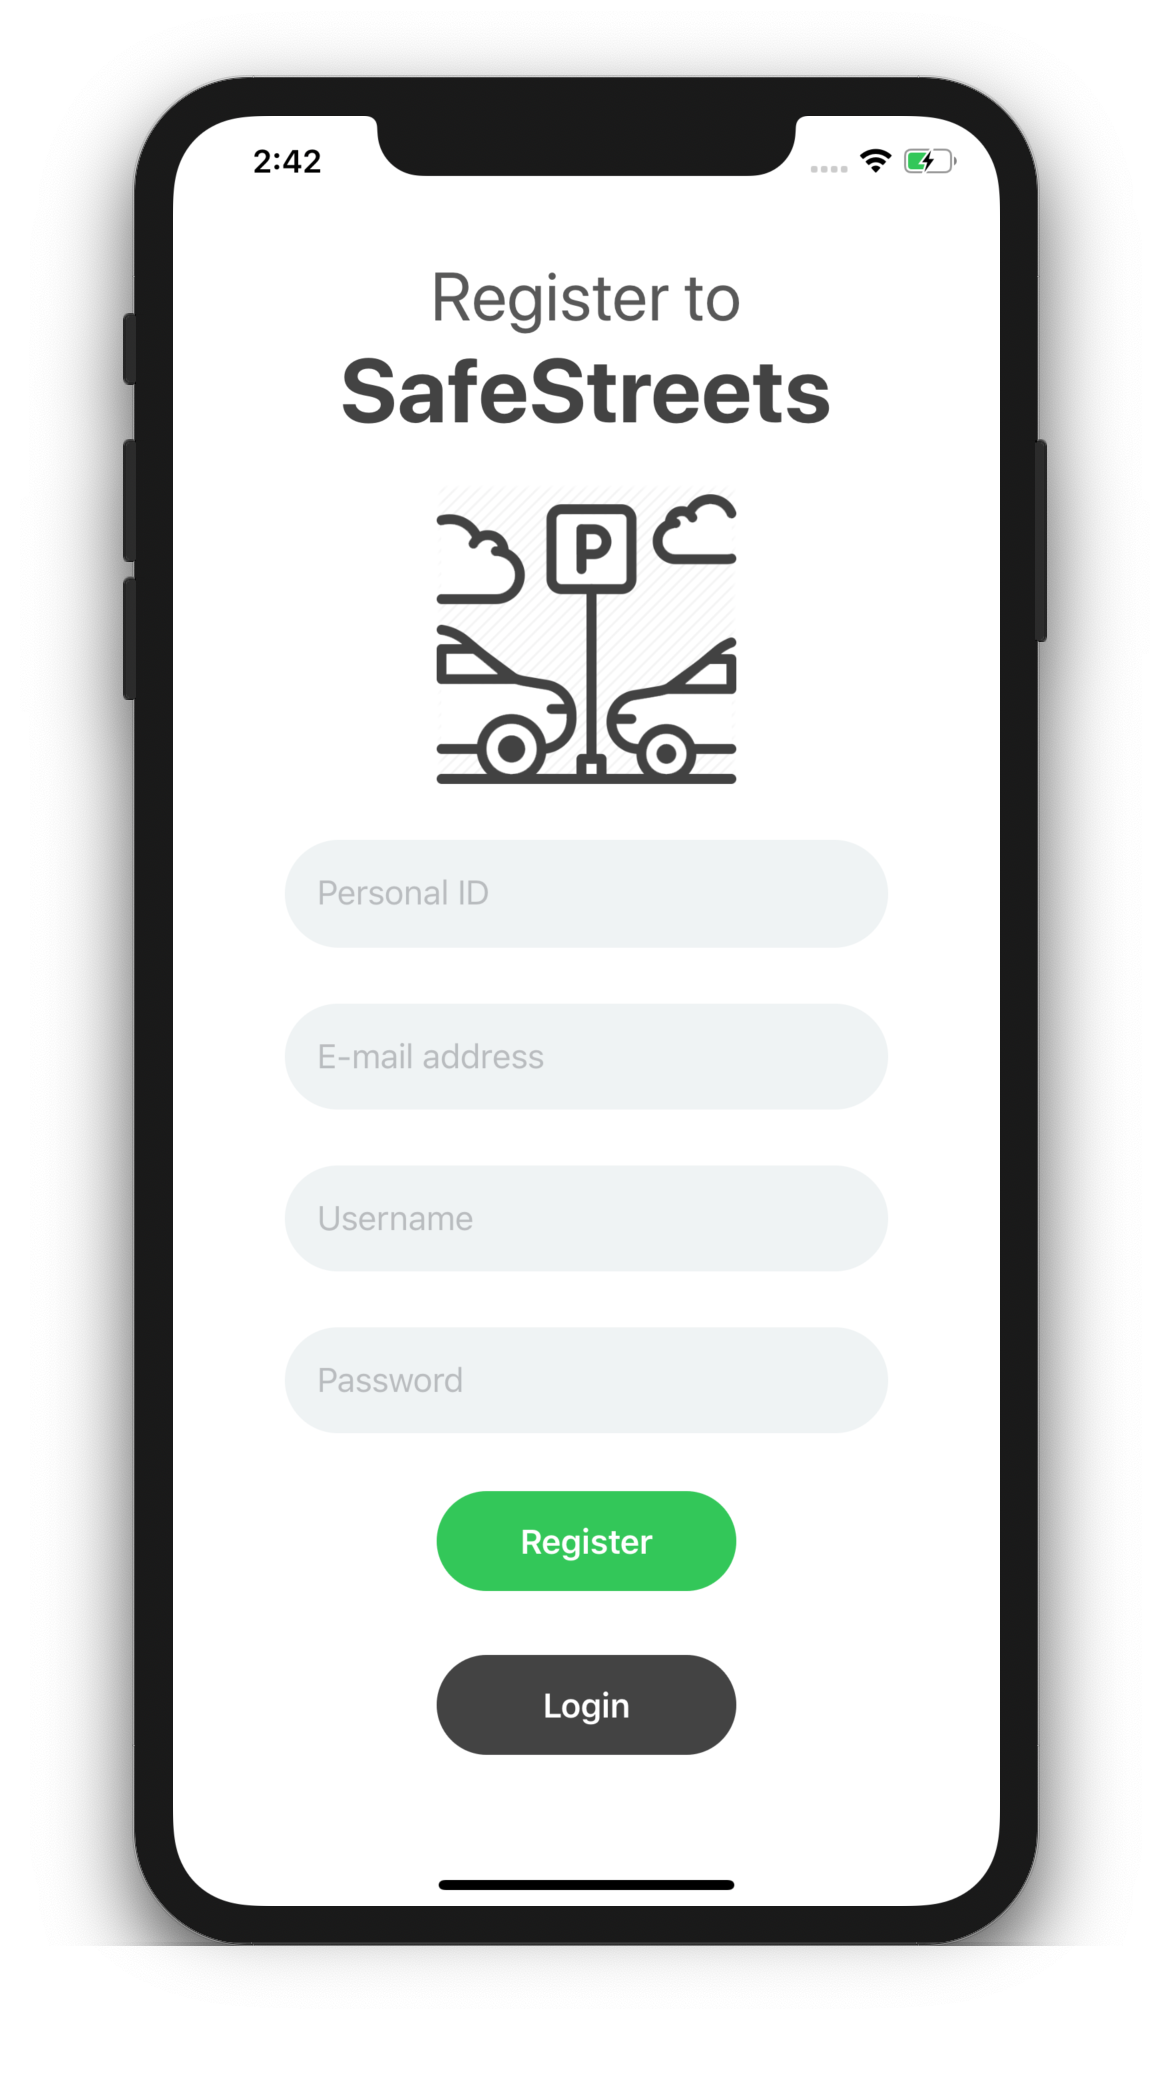
\includegraphics[width=\textwidth]{mockups/register-empty.png}
    					\caption{Registration Empty}
  				\end{minipage}
  				\hfill
  				\begin{minipage}[b]{0.4\textwidth}
    				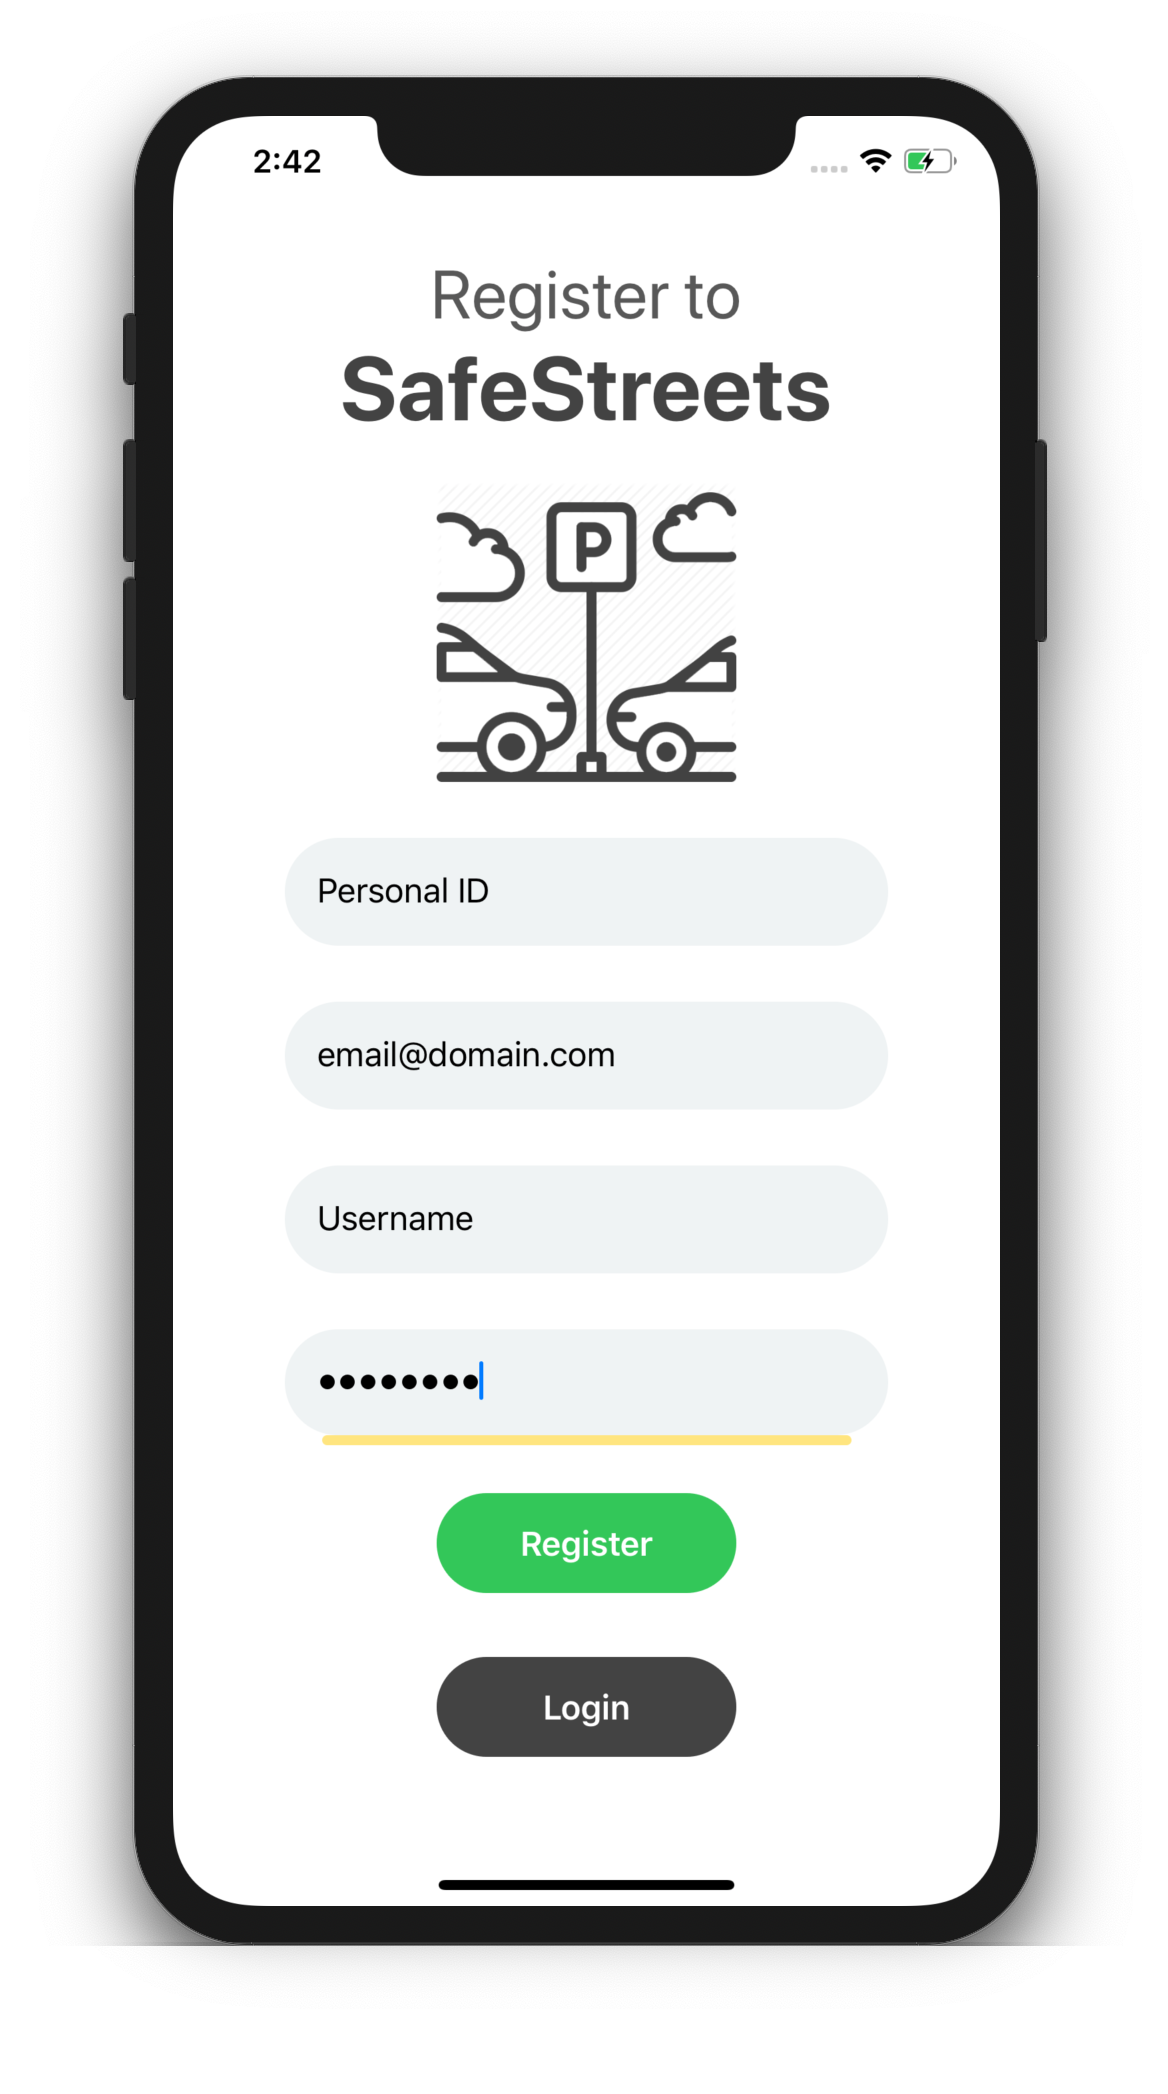
\includegraphics[width=\textwidth]{mockups/register.png}
    				\caption{Registration Filled}
  				\end{minipage}
			\end{figure}
		
			\begin{figure}[h]
  				\centering
  				\begin{minipage}[b]{0.4\textwidth}
    				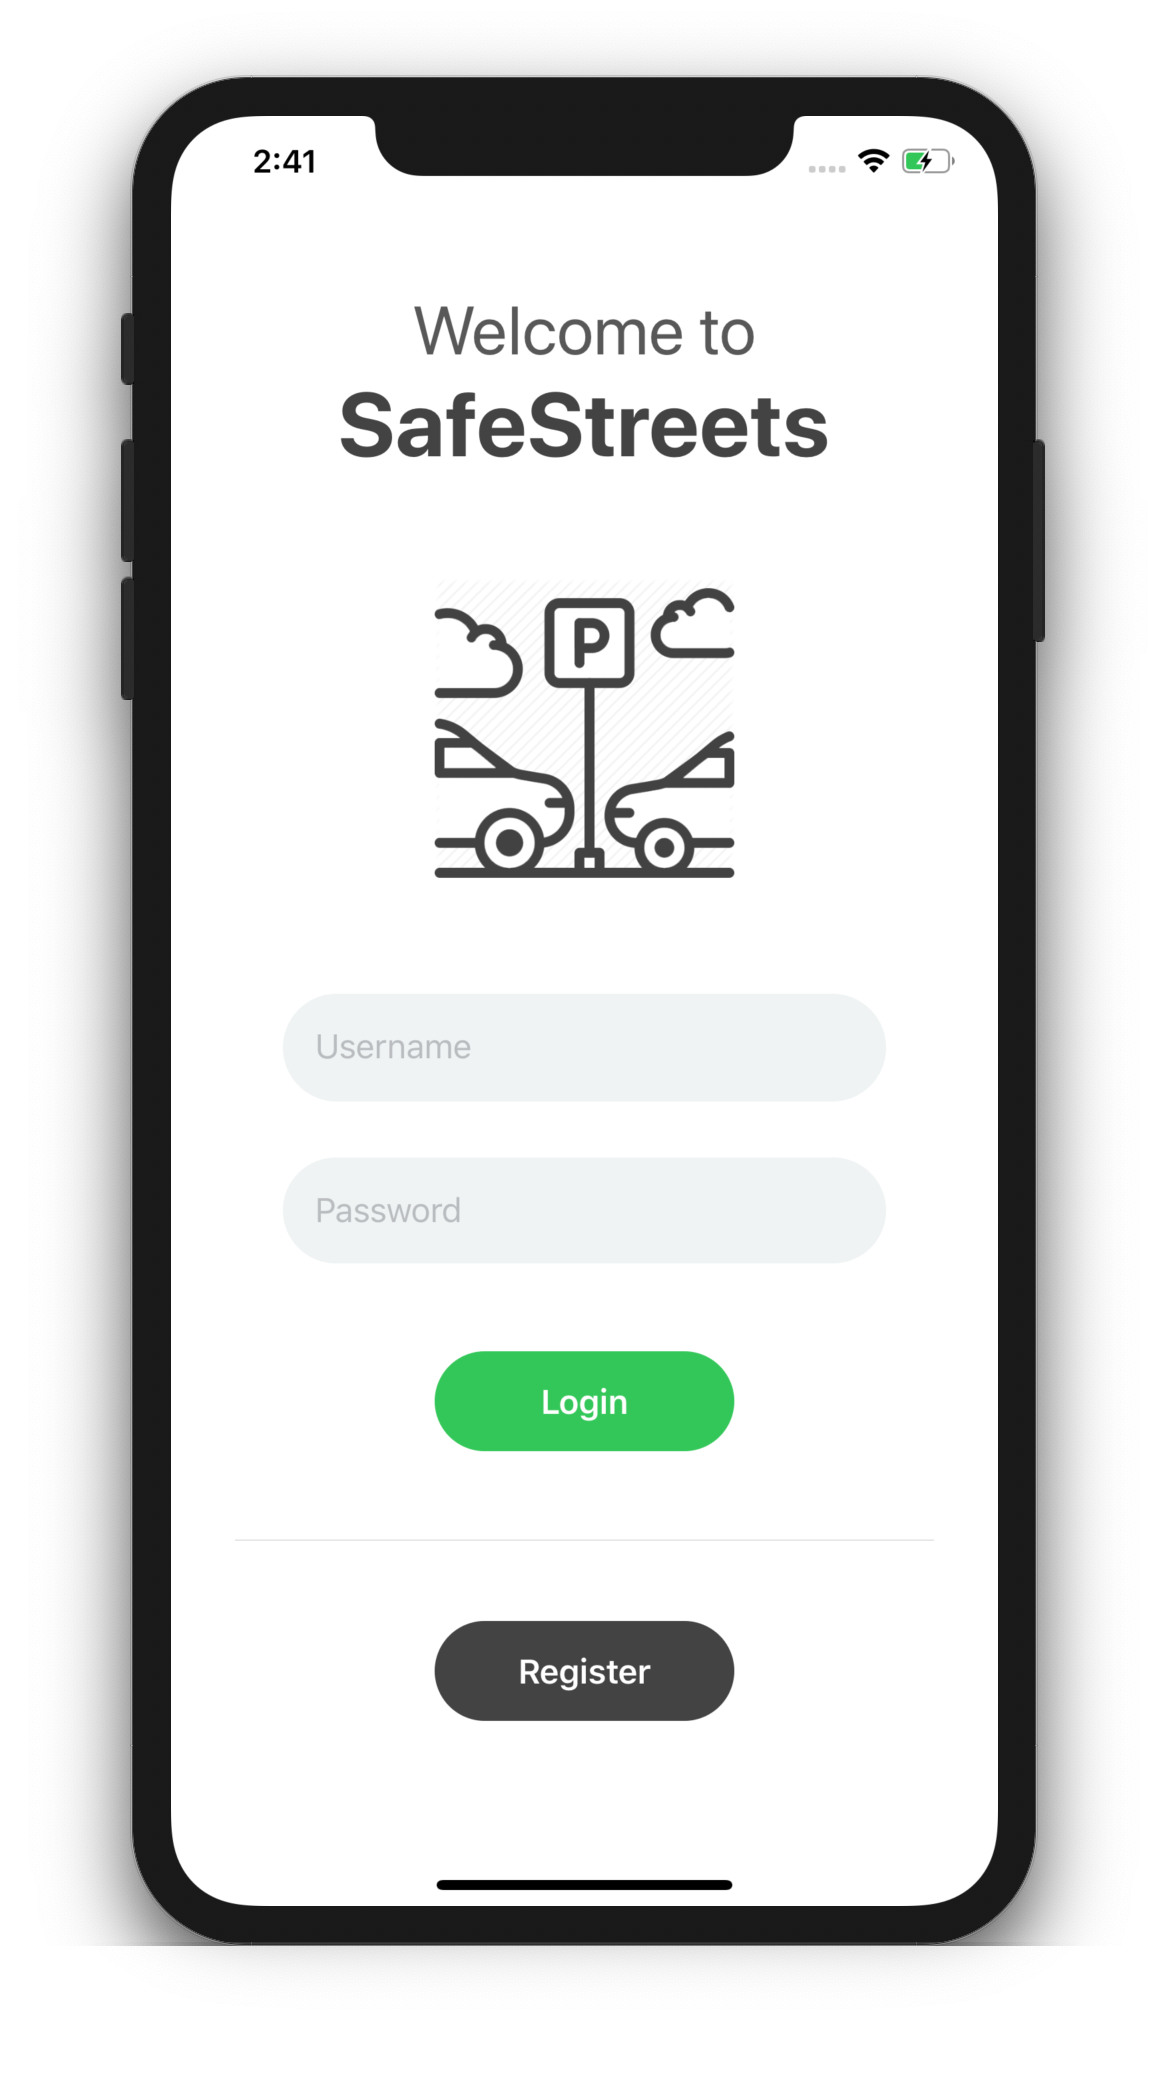
\includegraphics[width=\textwidth]{mockups/login-empty.png}
    					\caption{Login Empty}
  				\end{minipage}
  				\hfill
  				\begin{minipage}[b]{0.4\textwidth}
    				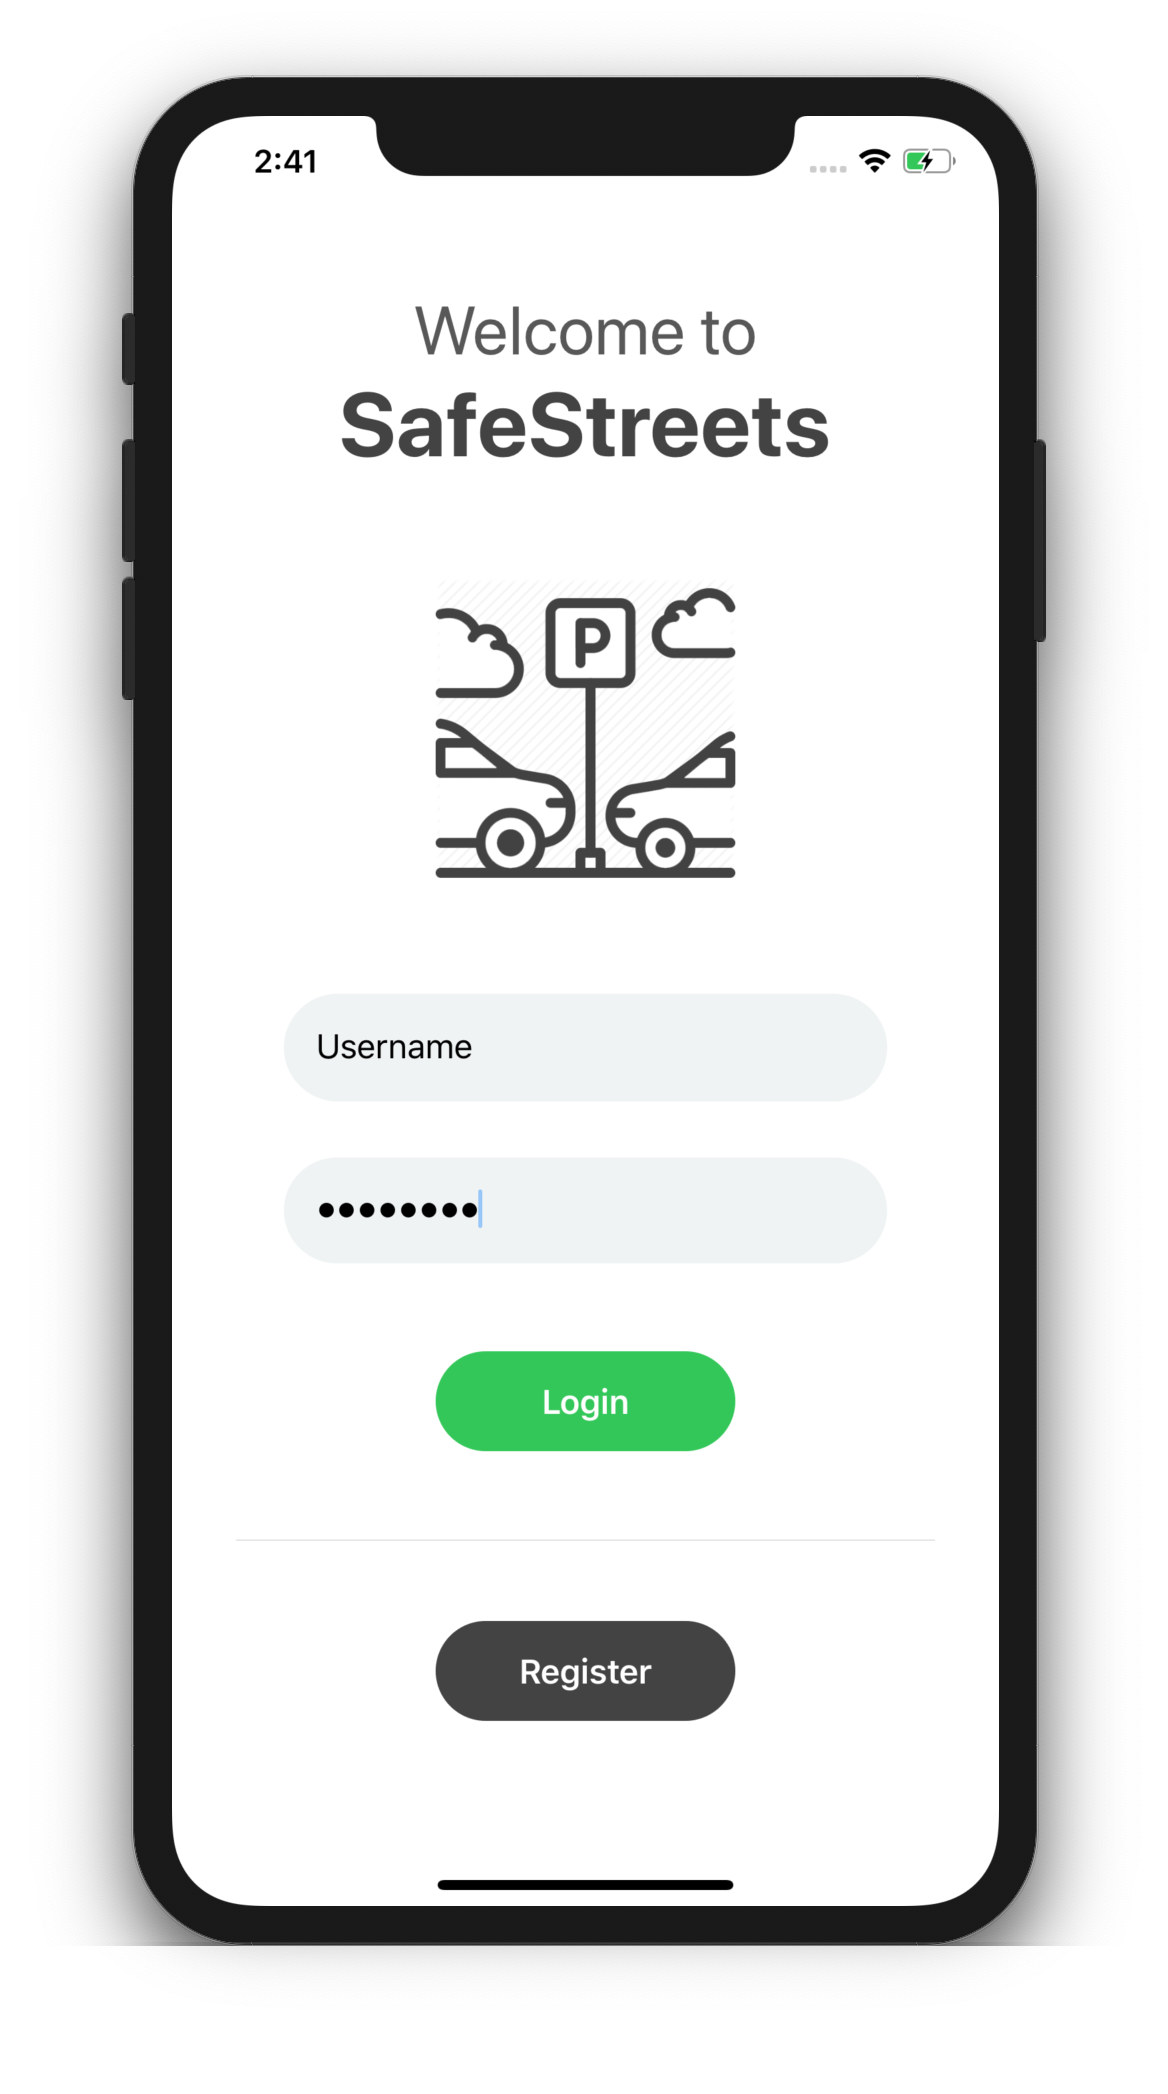
\includegraphics[width=\textwidth]{mockups/login.png}
    				\caption{Username Login}
  				\end{minipage}
			\end{figure}
			
	\end{itemize}



\newpage\paragraph{Logged User}
	\begin{itemize}
		\item The system is required to permit logged users to submit a violation. The submission is required to include a live photo captured via the \hyperref[sec:hardwareinterfaces]{hardware interfaces} of the user's device. The license plate number of the vehicle represented in the captured photo is not a mandatory field for the violation submission, but it will be leveraged for image recognition support if present. The user interface is required to allow the user to select the type of the committed violation from a predefined list of possible violations..			
		
		\item The system is required to allow logged users to consult a map through an external GIS and handle the different data visualisations discussed in the \hyperref[p:mde]{Municipality Data Exchange} section.
					 
			
			
		\item The system is required to allow logged users to consult the different statistics generated upon the system and the municipality collected data listed in the \hyperref[p:mde]{Geographic Information System} section.
		\item The system is required to allow logged users to view and edit the stored personal information in a profile section of the user interface and to log-out from the system. \newline\newline
			
			\begin{figure}[h]
  				\centering
  				\begin{minipage}[b]{0.4\textwidth}
    				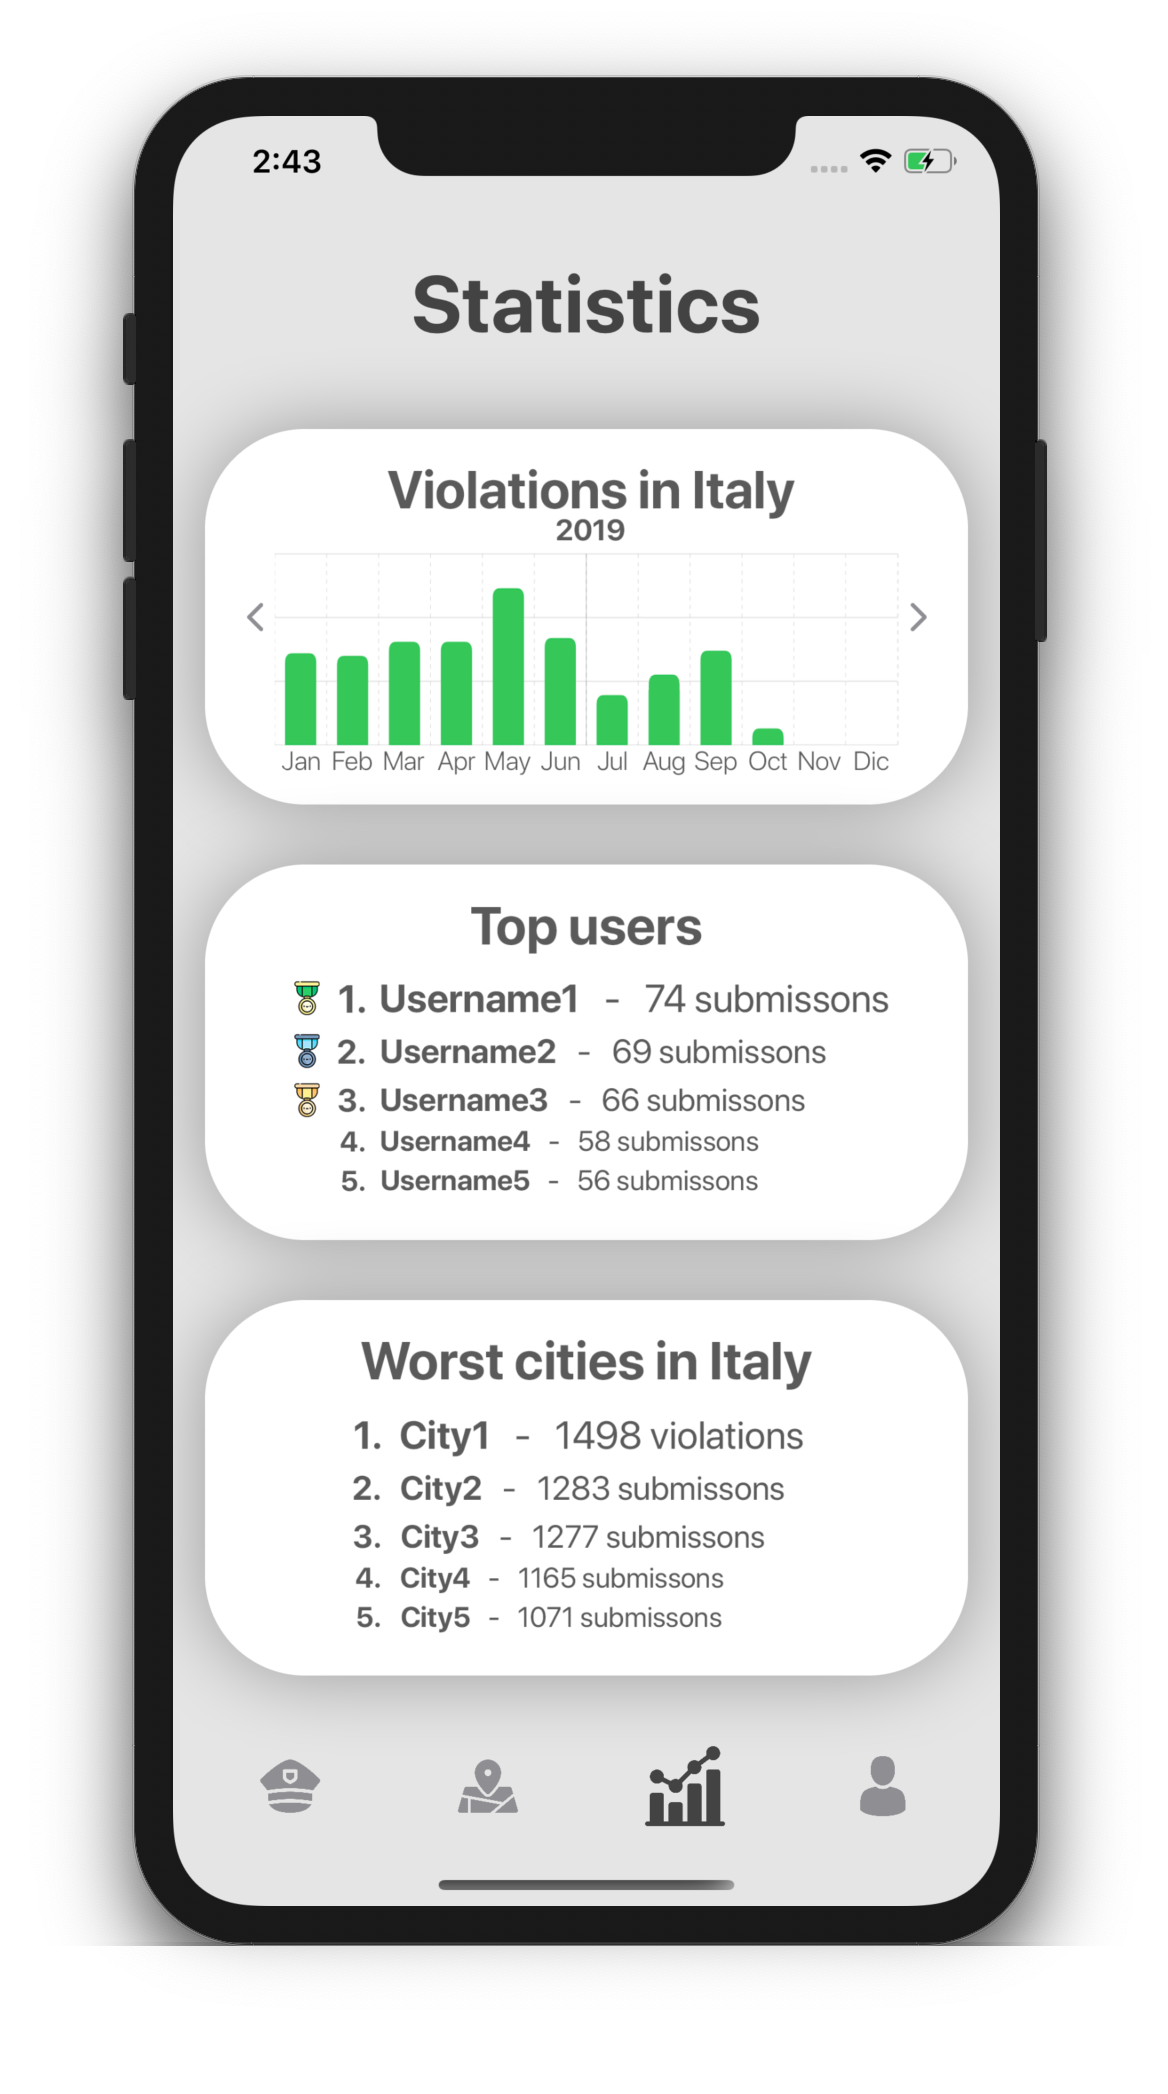
\includegraphics[width=\textwidth]{mockups/statistics.png}
    					\caption{Statistics View}
  				\end{minipage}
  				\hfill
  				\begin{minipage}[b]{0.4\textwidth}
    				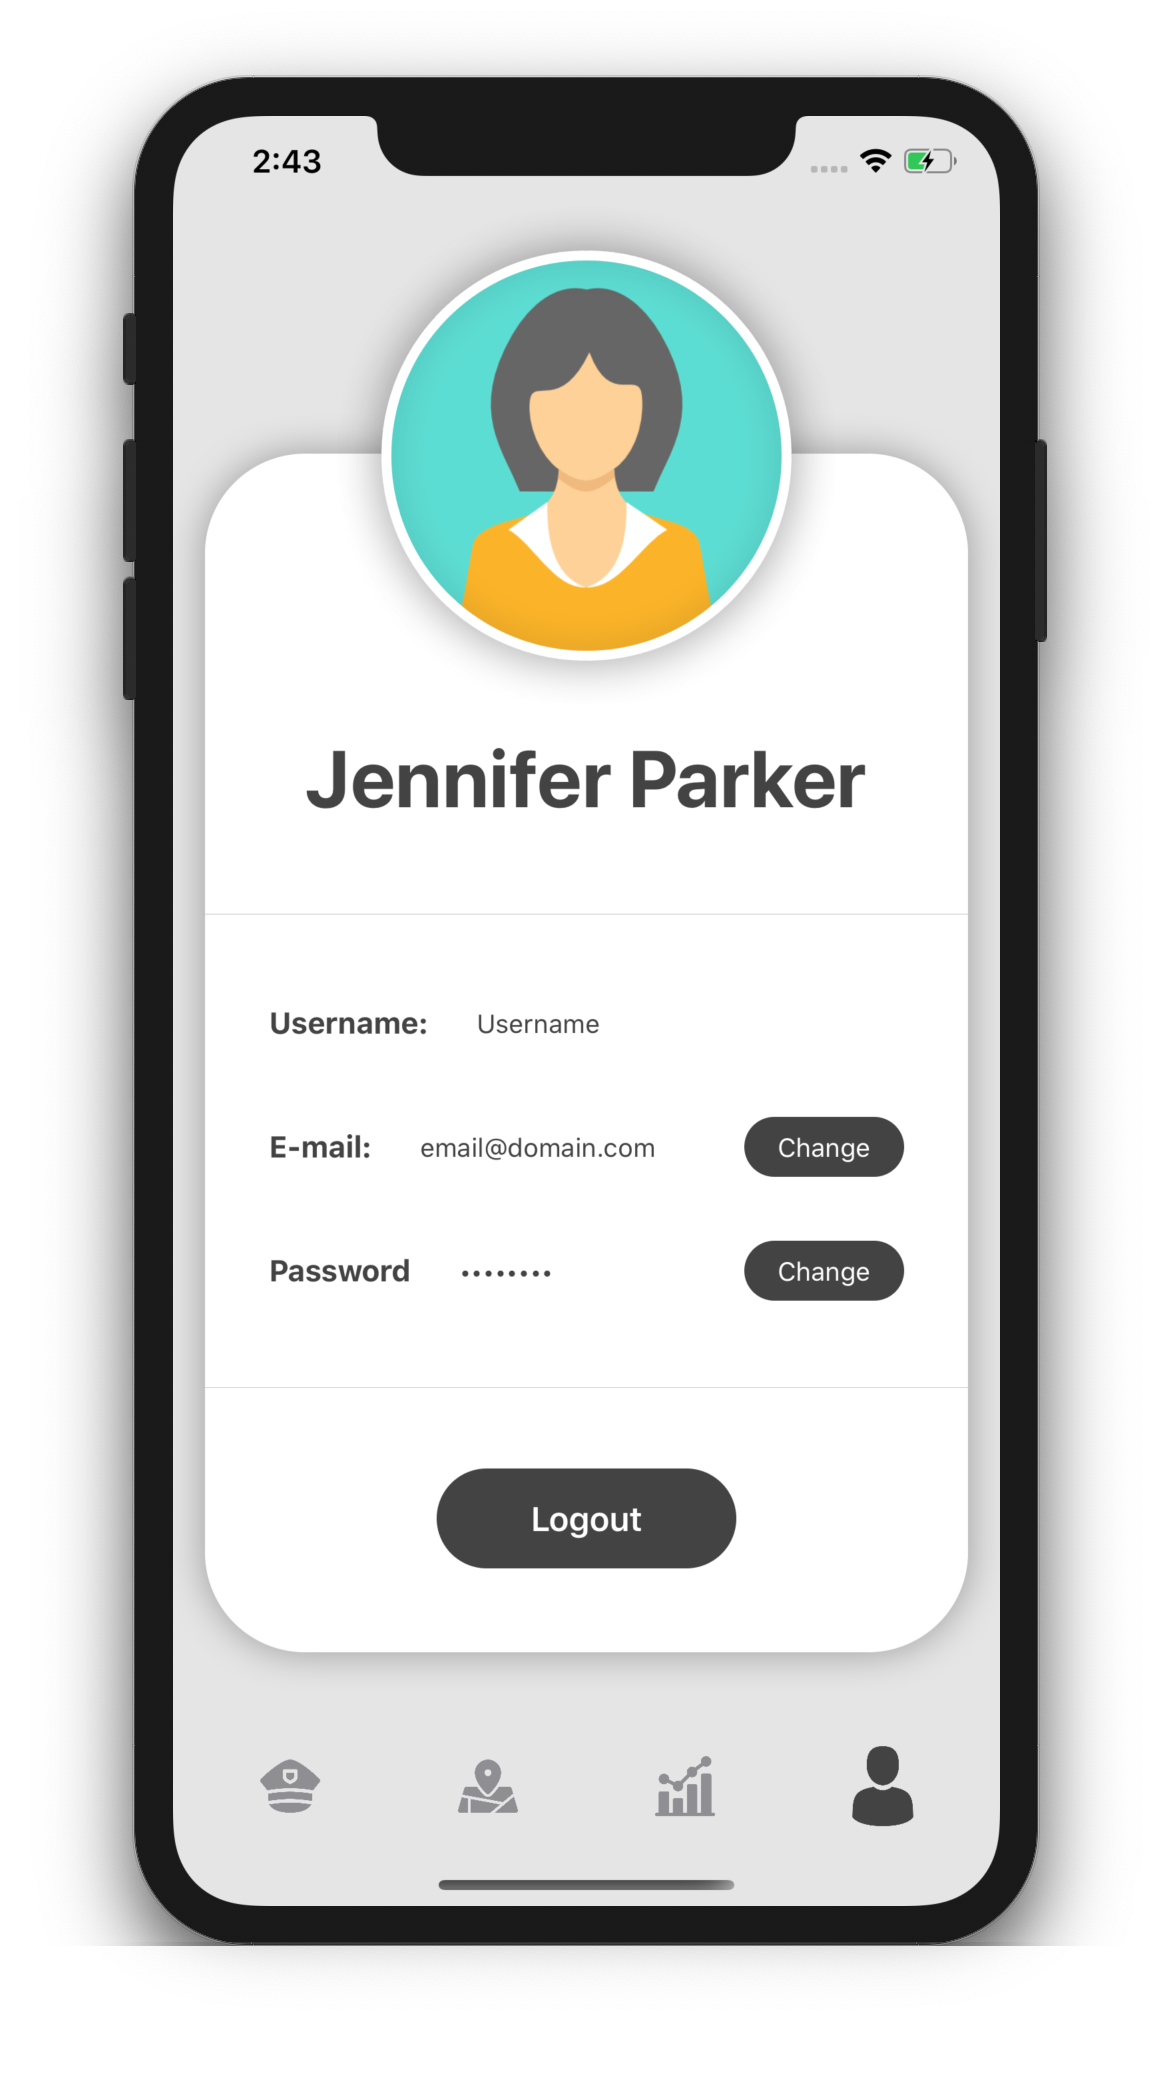
\includegraphics[width=\textwidth]{mockups/profile.png}
    				\caption{User Profile}
  				\end{minipage}
			\end{figure}
			
			\begin{figure}[h]
  				\centering
  				\begin{minipage}[b]{0.4\textwidth}
    				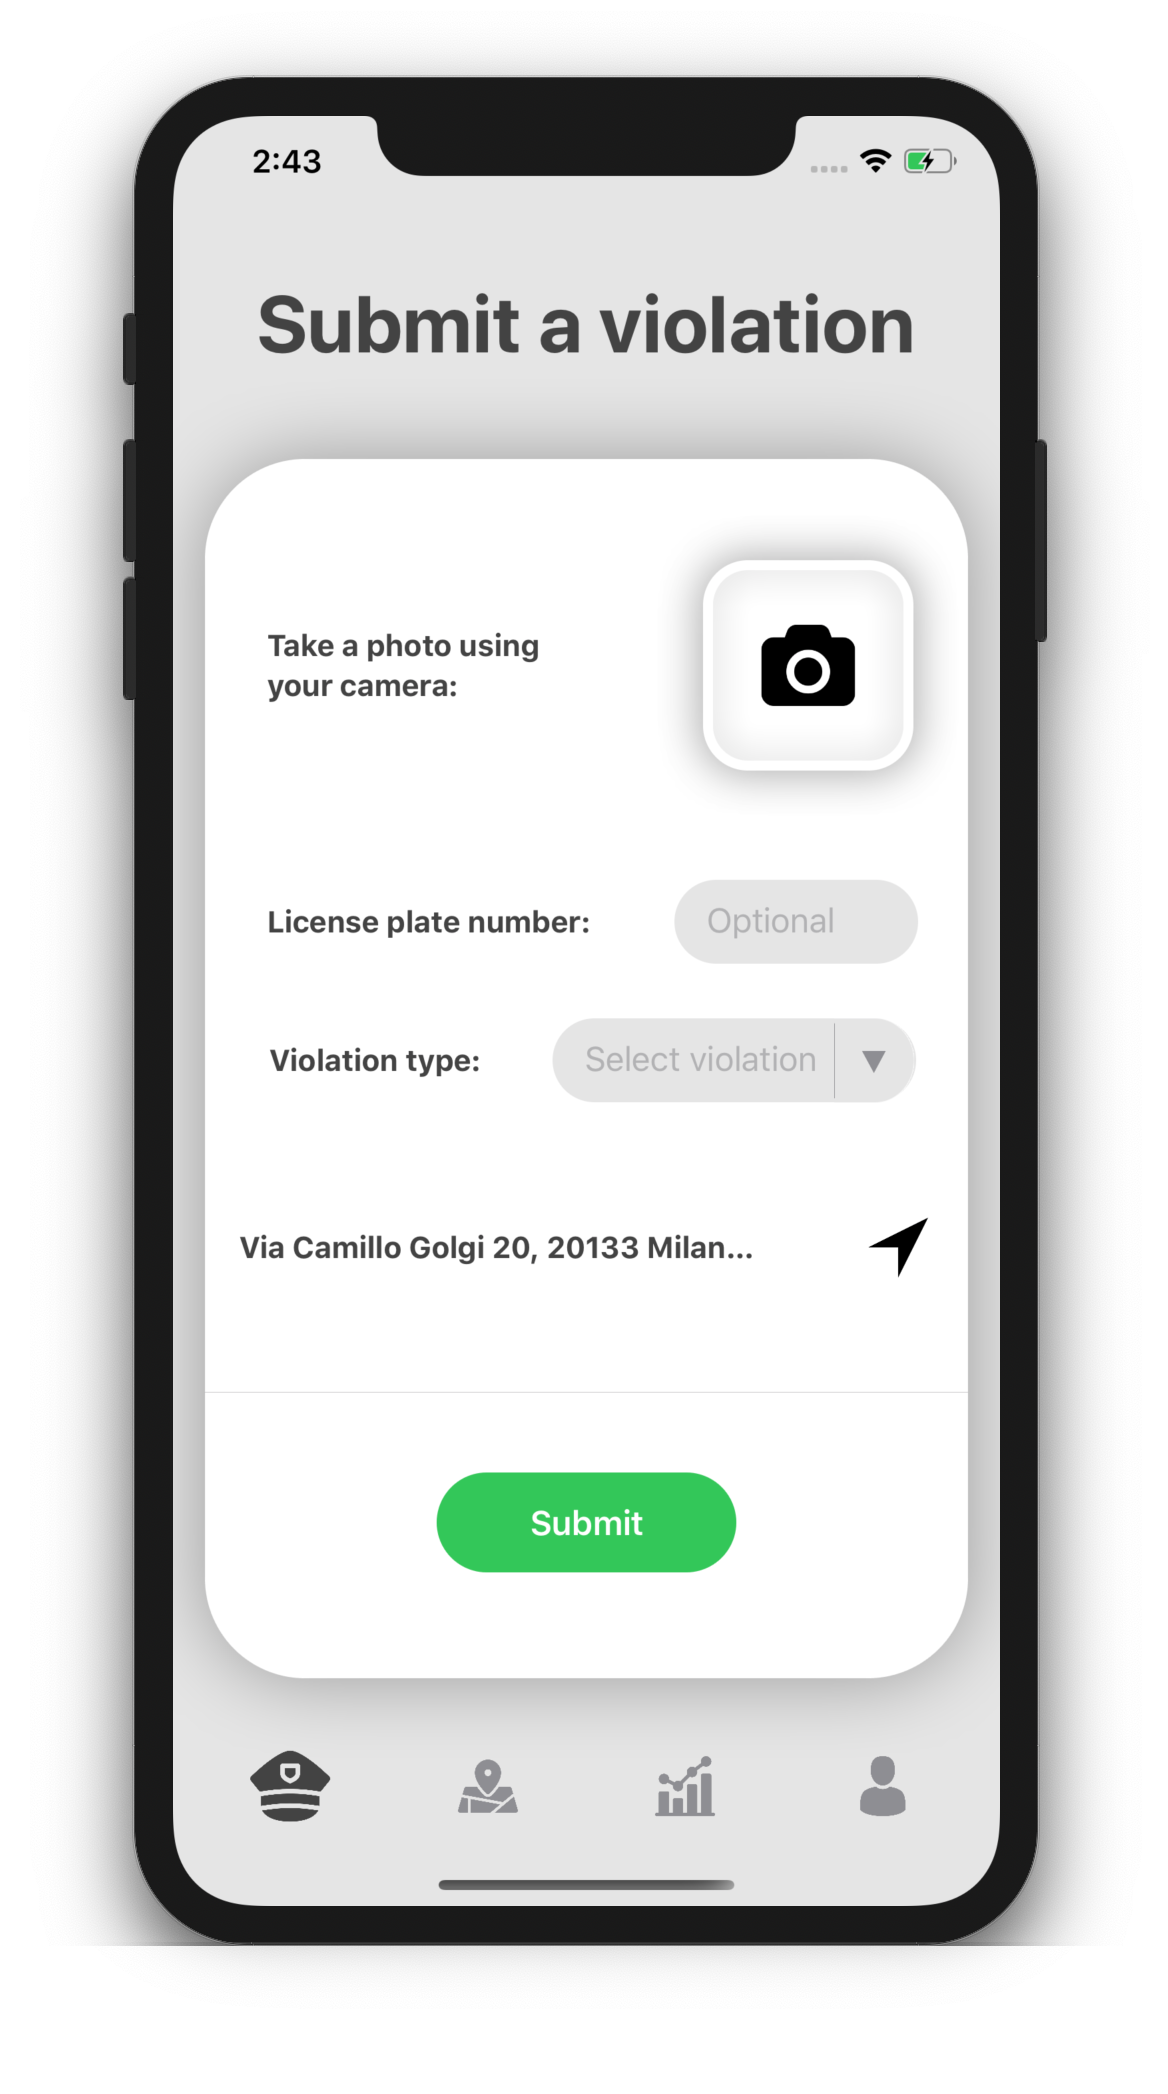
\includegraphics[width=\textwidth]{mockups/submit-violation.png}
    					\caption{Upload Procedure}
  				\end{minipage}
  				\hfill
  				\begin{minipage}[b]{0.4\textwidth}
    				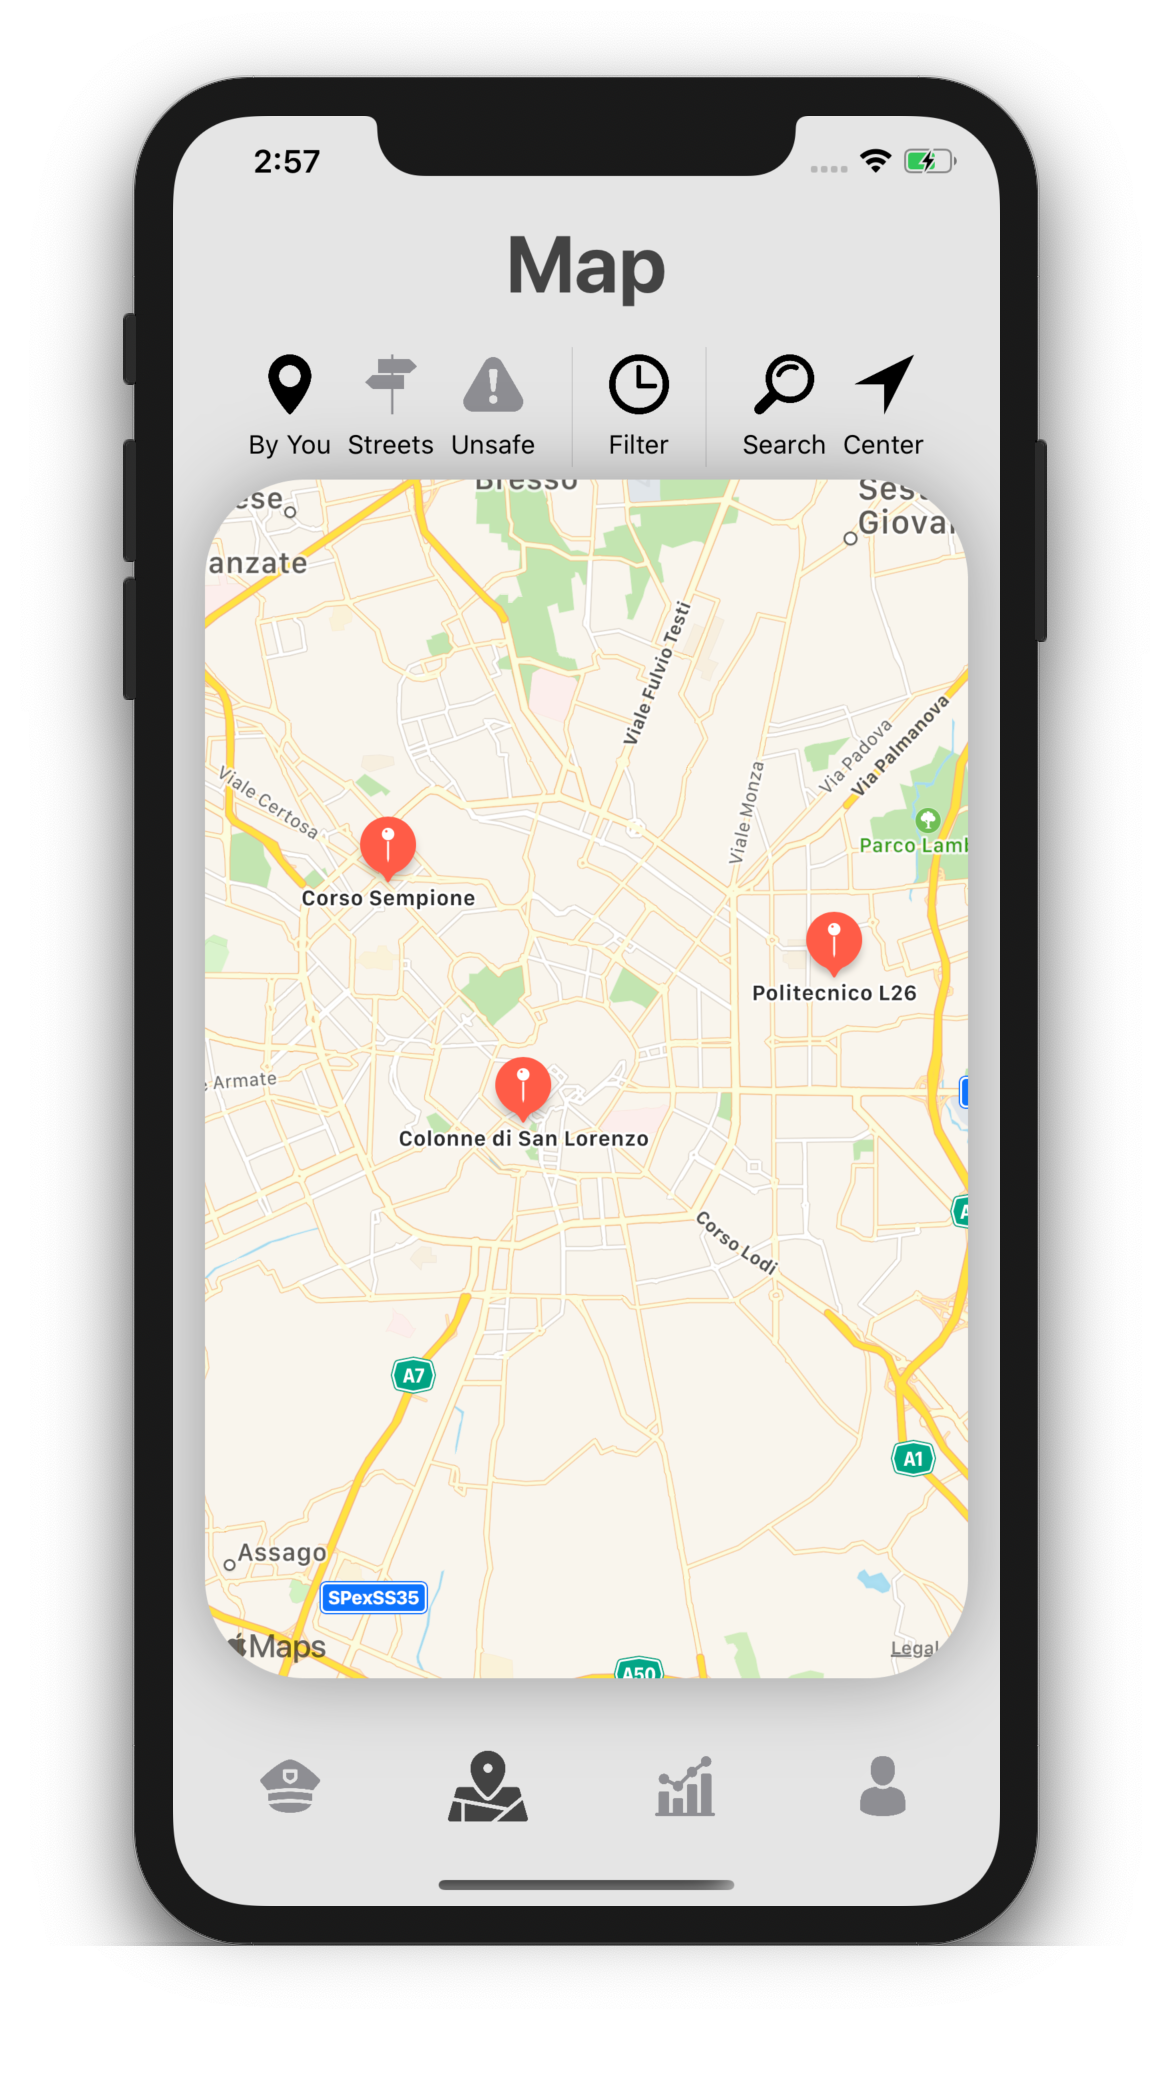
\includegraphics[width=\textwidth]{mockups/map.png}
    				\caption{Map Interface}
  				\end{minipage}
			\end{figure}
	\end{itemize}

\clearpage

\subsubsection{Hardware Interfaces}

The system will interact with the user's device hardware interfaces.	
	\begin{itemize} 
		\item Telephony and other wireless connections are leveraged for the communication between the user and the system
		\item Full access to the user's device camera hardware is needed for the user to capture a photo
		\item The geomagnetic field sensor and the proximity hardware-based sensor are leveraged to determine the position of the user's device
	\end{itemize}
	
\subsubsection{Software Interfaces}

TODO (Overall Description) In order to accomplish the \hyperref[sec:goals]{goals stated before} the system requires to interface with Databases and DBMSs, required in order to store data about users, violations, and the corresponding metadata. These interfaces are also required to guarantee the ability to input queries to the database in order to satisfy the system required capabilities.


\subsubsection{Communication Interfaces}

TODO (Overall Description) The system requires secure communication within the involved entities in a way not susceptible to eavesdropping or interception. Secure communication includes means by which the system can share information that third parties cannot intercept or alter. For these reasons communication encryption methods must be implemented in a way that guarantees the use of encryption, i.e. if encrypted communication is impossible then no traffic is sent.

\clearpage

\subsection{Functional Requirements}

\subsubsection{Scenarios}

Application specific scenarios are presented to enrich the system's specification. These scenarios describe the usage of the system.

\paragraph{Scenario 1}
\label{scenario:1}
	Davide is walking down the street while he notices a car parked over the crosswalks. He decides to open the SafeStreets app, register to the system with his fiscal code and submit the violation he just ran into. So he takes a picture from the in-app camera, he adds information such as the type of violation (i.e. "Bad Parking") and het allows his device integrated GPS to retrieve his current position, recognising the street in which the violation occurred. Finally, he submits the form, SafeStreet processes the uploaded data the authorities are alerted.

\paragraph{Scenario 2}
\label{scenario:2}
	Carlo wants to teach his son to drive but he doesn't want to expose him to difficult situations during his first experiences, so he decides to find the safest areas in Milan, where to lead his child driving. He opens the SafeStreets app and he consults the "Unsafe areas" section of the map, showing the most dangerous zones and the streets with the greatest number of accidents and violations. So Carlo is able to choose the roads he wants to avoid, assuring his son a safe drive.

\paragraph{Scenario 3}
\label{scenario:3}
	SafeStreets automatically retrieves data from the municipality service and, after processing the data about issued tickets, it notices that a restricted area of Milan is extremely often place of violations of cars parked in a prohibited zone. Thanks to a further analysis of the information provided by SafeStreets users, the pictures uploaded to the system highlight that the problem is a misleading signal, not allowing drivers to realise that they can't park in that area. SafeStreets contacts the municipality and notifies about this issue, suggesting a possible solution.

\paragraph{Scenario 4}
\label{scenario:4}
	The system receives a submission by a user alerting of a "Dangerously parked car". Processing the uploaded picture, it emerges that the vehicle is not completely placed within the stripes limiting the spots and, since the road where it was located is also crossed by railways, it is at risk of a collision with a train. SafeStreets alerts the authorities in order to anticipate and facilitate the car removal and the resulting ticket emission, possibly avoiding an accident.	
	
\paragraph{Scenario 5}
\label{scenario:5}
	Eleonora is about to leave for a trip to Italy with her friends, but they are undecided on which means of transport to choose, between moving by car or traveling by train, taking advantage of the local transport means of each city. Opening the SafeStreets app and consulting its Statistics section, they find out that the cities they want to visit are among the most subject to violations, meaning that it could turn out hard driving in their destinations, so they decide to leave by train.
	
\clearpage

\subsubsection{Use Case Diagram}
	\begin{figure}[h!]
		\centering
		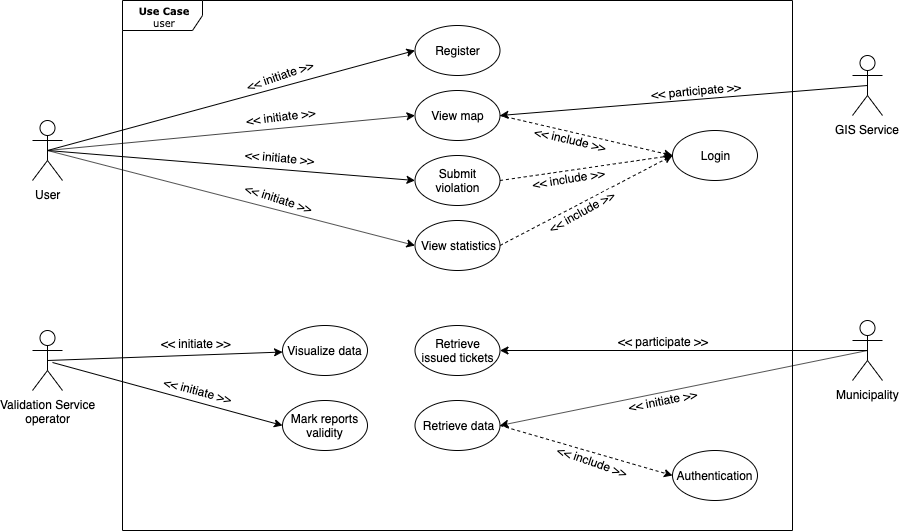
\includegraphics[width=\linewidth]{diagrams/UseCaseDiagram.png}
		\caption{
			\label{fig:useCase} 
				Use case diagram
		}
	\end{figure}
	
	\paragraph{Notes to read the diagram}
	\begin{itemize}
		\item The use case diagram represents the possible interactions of actors with the system and the different use cases in which the actors are involved.

		\item The "Municipality" actor includes all the authorities having access to the system, both to consult SafeStreets information and to retrieve data from the provided API.
		
		\item Since the API has a restricted access, the authority must authenticate to the system in order to retrieve data from it.
		
		\item Authorities don't participate in the registration process because they login with a given account.
		
		\item The "GIS Service" is the external Geographical Information System used for the Map service integration.
	\end{itemize}
		

\clearpage

\subsubsection{Use Cases Description}

\textbf{Registration}

\begin{longtable}{p{0.25\linewidth}p{0.75\linewidth}}
\toprule
\textbf{Name} & \textbf{Registration} \\
\midrule
\textbf{Actors} & Guest user \\
\midrule
\textbf{Entry\newline conditions} &  The guest user downloaded and opened the app\\
\midrule
\textbf{Flow of events} & 
\begin{enumerate}
	\item The user asks the system to register to its services
	\item The system shows the appropriate form to fill to register to the system
	\item The user inserts his personal ID to verify his identity
	\item The user inserts his own email address
	\item The user inserts a username to be uniquely identified by the system
	\item The user inserts a password accordingly to the security constraints
	\item The user confirms data inserted are correct e submit the form
	\item The system checks the personal ID isn't already registered
	\item The system checks the username to be unique
	\item The system checks the email to be unique
	\item The system sends an email to the user with a unique link to verify the email address inserted by the user really belongs to him
	\item The user clicking on the link received confirms his email address
	\item The user is notified by mail the registration procedure is correctly completed
\end{enumerate} \\

\midrule

\textbf{Exit conditions} & The user is able to login to the system as a \emph{registered} user with its own credentials\\
\midrule
\textbf{Exceptions} & 
\begin{itemize}
	\item If the personal ID inserted by the user is already registered, the system displays an error message asking the user to recover his account
	\item If the username inserted by the user is already taken by another user, the system displays an error message asking the user to insert another username
	\item If the email inserted by the user is already used by another user, the system displays an error message asking the user to insert another email address
	\item If the user notices to have entered wrong informations he could edit them at the end of the process of registration in his personal page
\end{itemize} \\
\bottomrule
\caption{\emph{Registration} use case description}
\end{longtable}

\begin{figure}[h!]
	\centering
	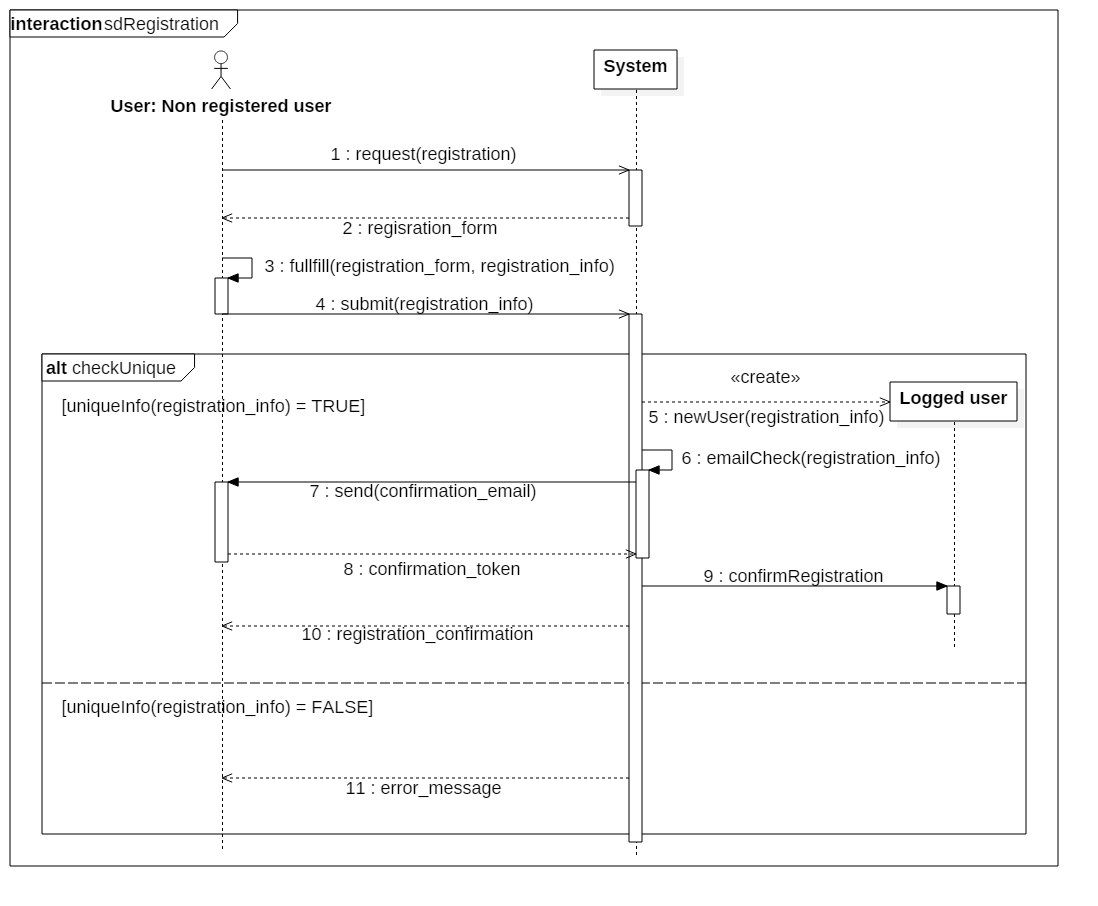
\includegraphics [width=\textwidth]{diagrams/sdRegistration.png}
	\caption{
		\label{fig:registrationSequence} 
		\emph{Registration} sequence diagram
	}
\end{figure}

\clearpage

\textbf{Login}
\begin{longtable}{p{0.25\linewidth}p{0.75\linewidth}}
\toprule
\textbf{Name} & \textbf{Login} \\
\midrule
\textbf{Actors} &  Registered user \\
\midrule
\textbf{Entry \newline conditions} & The user must know his username and password \\
\midrule
\textbf{Flow of events} & 
\begin{enumerate}
	\item The user inserts his username and password in the appropriate form and submit it
	\item The system validates the inserted credentials checking also if the user has confirmed his own email address
\end{enumerate} \\
\midrule
\textbf{Exit conditions} & If the credential validation is successful, user is successfully logged in\\
\midrule
\textbf{Exceptions} & 
\begin{itemize}
	\item If the credential validation failed, an error message is displayed
	\item If the credential validation is successful but the email address isn't confirmed, the user is reminded to validate it through the received confirmation email
\end{itemize} \\
\bottomrule
\caption{\emph{Login} use case description}
\end{longtable}


\begin{figure}[h!]
	\centering
	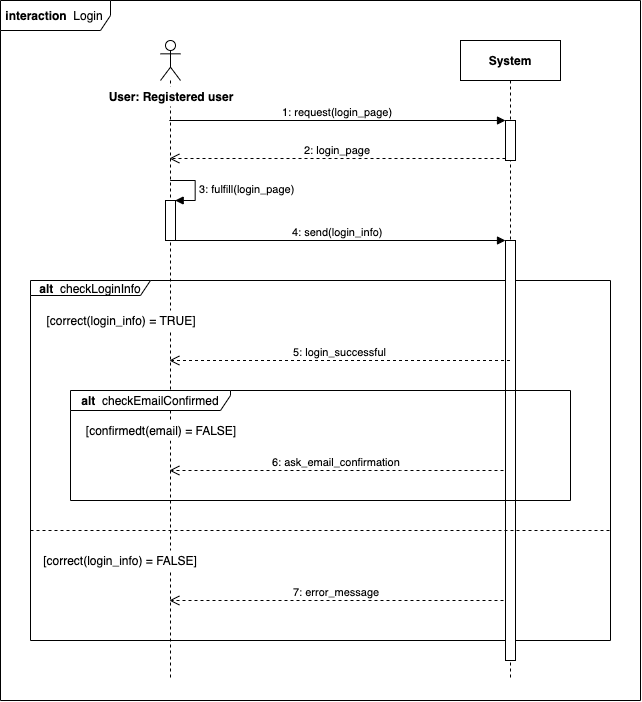
\includegraphics [width=\textwidth]{diagrams/sdLogin.png}
	\caption{
		\label{fig:loginSequence} 
		\emph{Login} sequence diagram
	}
\end{figure}

\clearpage

\textbf{API Authentication}
\begin{longtable}{p{0.25\linewidth}p{0.75\linewidth}}
\toprule
\textbf{Name} & \textbf{Authentication} \\
\midrule
\textbf{Actors} &  Municipality \\
\midrule
\textbf{Entry \newline conditions} & The authority must know his username and password \\
\midrule
\textbf{Flow of events} & 
\begin{enumerate}
	\item The authority user inserts his username and password in the appropriate form and submit it
	\item The system validates the inserted credentials
\end{enumerate} \\
\midrule
\textbf{Exit conditions} & If the credential validation is successful, access to the API is given to the authority\\
\midrule
\textbf{Exceptions} & 
\begin{itemize}
	\item If the credential validation failed, an error message is displayed
	\item If the entered username is invalid, the municipality is prompted to manually contact the system owners to request a specific account to access the API functionalities
\end{itemize} \\
\bottomrule
\caption{\emph{API Authentication} use case description}
\end{longtable}

\begin{figure}[h!]
	\centering
	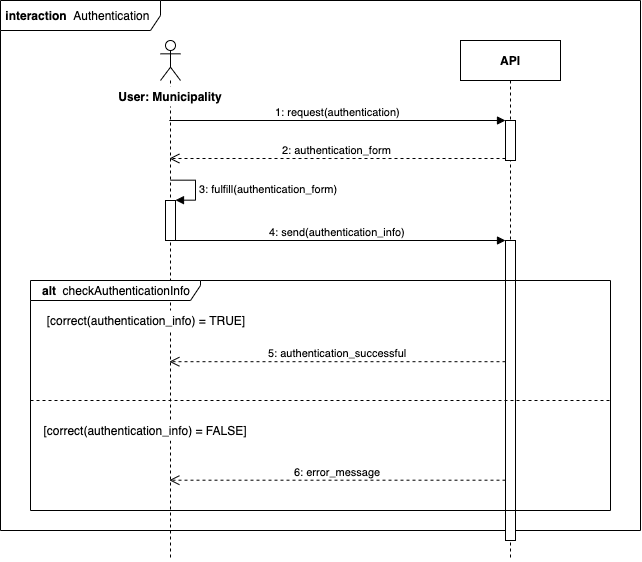
\includegraphics [width=\textwidth]{diagrams/sdAuthentication.png}
	\caption{
		\label{fig:authSequence} 
		\emph{API Authentication} sequence diagram
	}
\end{figure}

\clearpage

\textbf{Violation Submission}
\begin{longtable}{p{0.25\linewidth}p{0.75\linewidth}}
\toprule
\textbf{Name} & \textbf{Violation Submission} \\
\midrule
\textbf{Actors} &  Logged user \\
\midrule
\textbf{Entry \newline conditions} & The user is logged in \\
\midrule
\textbf{Flow of events} & 
\begin{enumerate}
	\item The user takes a picture portraying the violation, with the license plate of the vehicle clearly visible
	\item The user selects the most suitable violation type
	\item The user possibly enters the license plate number manually
	\item The user allows the app to retrieve his current location using the device GPS
	\item The submits the fulfilled form
	\item The system starts processing the entered information the picture, recognising the license plate number
	\item The system registers the violation
	\item The system confirms the procedure success
\end{enumerate} \\
\midrule
\textbf{Exit conditions} & The user has successfully submitted the violation\\
\midrule
\textbf{Exceptions} & 
\begin{itemize}
	\item If a problem retrieving the current user location occurs, the user is warned to check the GPS service is accessible
	\item If an upload problem occurs, the user is warned to check the internet connection
	\item If the system cannot retrieve the license plate number and it isn't manually specified or the numbers don't match, an error is reported to the user
\end{itemize} \\
\bottomrule
\caption{\emph{Violation Submission} use case description}
\end{longtable}

\begin{figure}[h!]
	\centering
	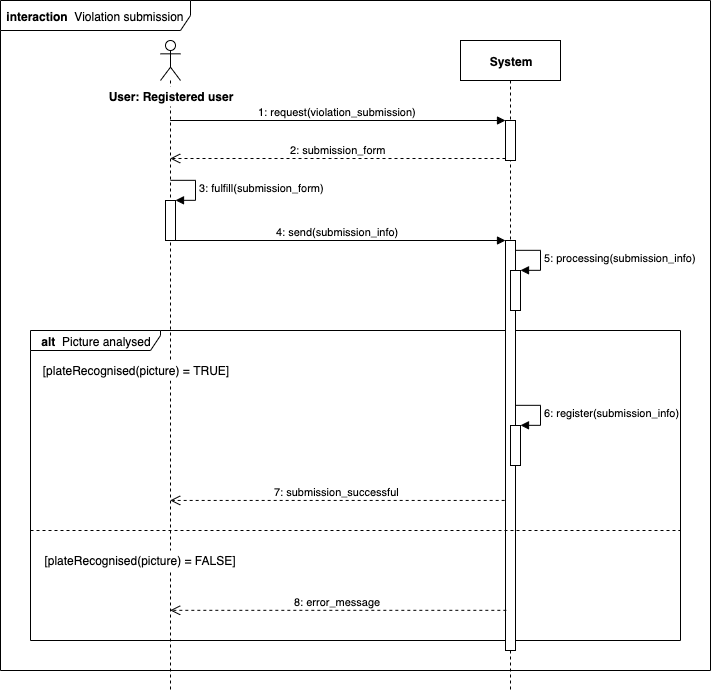
\includegraphics [width=\textwidth]{diagrams/sdViolationSubmission.png}
	\caption{
		\label{fig:submissionSequence} 
		\emph{Violation Submission} sequence diagram
	}
\end{figure}

\clearpage

\clearpage
\textbf{View Map}
\begin{longtable}{p{0.25\linewidth}p{0.75\linewidth}}
\toprule
\textbf{Name} & \textbf{View Map} \\
\midrule
\textbf{Actors} & Logged user \\
\midrule
\textbf{Entry \newline conditions} & The user is logged in \\
\midrule
\textbf{Flow of events} & 
\begin{enumerate}
	\item The user chooses the type of map he wants to consult among:
		\subitem a1. The map with his previously submitted violations
		\subitem a2. The map with all the submitted violations
		\subitem a3. The map highlighting the safe and unsafe areas
	\item The user possibly selects the time interval of the violations he wants to view
	\item The user sends the request
	\item The system retrieves the map from the GIS Service
	\item The system enriches the retrieved map with the requested information
	\item The system shows the map in the user's instance of the app
\end{enumerate}\\
\midrule
\textbf{Exit conditions} & The user can view and explore the map\\
\midrule
\textbf{Exceptions} & 
\begin{itemize}
	\item If the selected time interval is invalid, the user is warned and prompted to select a valid one
	\item If the GIS Service cannot be retrieved, an error is reported to the user
\end{itemize} \\
\bottomrule
\caption{\emph{View Map} use case description}
\end{longtable}

\begin{figure}[h!]
	\centering
	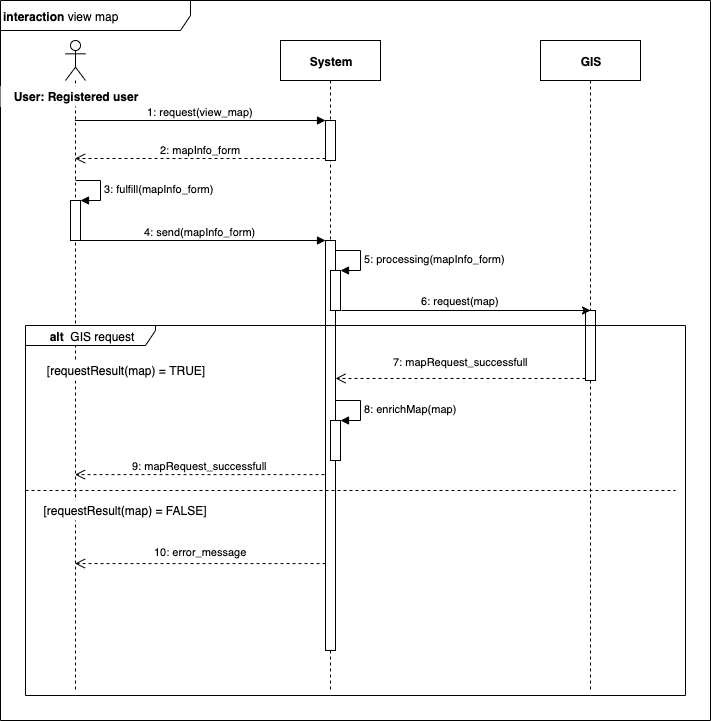
\includegraphics [width=\textwidth]{diagrams/sdViewMap.png}
	\caption{
		\label{fig:mapSequence} 
		\emph{View Map} sequence diagram
	}
\end{figure}

\clearpage

\subsubsection{Requirements Mapping}

	The following requirements are derived in order to achieve the specified goals.
	\begin{description}
		\item \ref{goal:register} Allow guest users to register to the system
			\begin{enumerate}[label=\textbf{R\arabic*}]
			
  				\item The system must require the \emph{guest} user to insert his fiscal code, a username, a valid e-mail and a password to identify him
  				
   				\item The system must check that the validity of the data inserted by the \emph{guest} user namely avoid duplicates, invalid fiscal codes and too weak passwords
   				
   				\item The system must send an e-mail to the \emph{guest} user to verify the e-mail address given during the registration
   
  			\end{enumerate}
  				
			\textbf{\ref{assumption:workingConnection}} Internet connection always works correctly
			
			\textbf{\ref{assumption:workingDBMS}} The DBMS always works properly so that the information in the DB are always accessible
			
			\textbf{\ref{assumption:smartphoneOS}} The smartphone of the user runs iOS (9 or later) or Android (Jelly Bean or later) \newline
			
  			
		\item \ref{goal:login}\ Allow registered users to authenticate to the system
			\begin{enumerate}[label=\textbf{R\arabic*}, resume]
  				\item The system must require the user to insert his username and password to authenticate to the system
   				\item The system must be able to check if the username and password pair correspond to a user correctly registered to the system and grant the access to that user 
			\end{enumerate}
			
			\textbf{\ref{assumption:workingConnection}} Internet connection always works correctly
			
			\textbf{\ref{assumption:workingDBMS}} The DBMS always works properly so that the information in the DB are always accessible \newline
			
		\item \ref{goal:userTransfer}\ Allow users to transfer data to the system describing occurred violations, including the suitable metadata to describe the submitted violation			
			 \begin{enumerate}[resume*]
				\item The system must allow the user to take a picture of the violation and the plate from the mobile application
  				\item The system must allow the user to manually insert the license plate number in order to help the recognition algorithm
  				\item The system must be able to retrieve the license plate of the vehicle running an algorithm to recognise it
  				\item The system must be able to verify that the license plate number is valid and registered to a vehicle
  				\item The system must require the user to specify the type of violation
  				\item The system must allow the user to provide the location of the violation, manually specifying the address, picking it up from the map or using the GPS of the device
   			\end{enumerate}
   			
   			\textbf{\ref{constraint:pictureQuality}} The quality of the picture is sufficient to recognise the plate number (min resolution 320x240)
   			
			\textbf{\ref{constraint:strongConnection}} Internet connection must be strong enough to allow the upload of the picture in a reasonable amount of time (supported technologies are 3G, 4G and 5G due to the performance requirement)
			
			\textbf{\ref{assumption:obtainableGPS}} GPS position of all users is always obtainable
			
			\textbf{\ref{assumption:workingConnection}} Internet connection always works correctly
			
			\textbf{\ref{assumption:workingDBMS}} The DBMS always works properly so that the information in the DB are always accessible \newline
			
		\item \ref{goal:avoidLeaks}\ Ensure that the chain of custody of the information provided by the users is never broken, and the information is never altered or manipulated			
			\begin{enumerate}[resume*]
   				\item The system must provide a secure channel to communicate with the users
   				\item The system must encrypt the connection with the users in order to protect the process of providing data
   				\item The system must adopt security measures to prevent malicious accesses and to protect sensible data
   				\item Questo davvero non lo so mori miei
  			\end{enumerate}
			\textbf{\ref{assumption:workingConnection}} Internet connection always works correctly \newline
			
		\item \ref{goal:municipalityTransfer}\ Allow the system to retrieve data about the accidents that occur on the territory and data about issued tickets via the municipality provided service
			\begin{enumerate}[resume*]
   				\item The system must be able to retrieve data about accidents from municipality systems 
   				\item The system must be able to process data retrieved from municipality
   				\item The system must be able to elaborate accidents and violations information to extract data about unsafe areas
   				\item The system must be able to provide data to municipality systems to suggest possible interventions to increase safety in a specific area
  			\end{enumerate}
  			
  			\textbf{\ref{assumption:workingConnection}} Internet connection always works correctly
  			
			\textbf{\ref{assumption:municipalityReachable}} Municipality services are always reachable
			
  			\textbf{\ref{assumption:workingDBMS}} The DBMS always works properly so that the information in the DB are always accessible \newline
  			
  		\item \ref{goal:statistics}\ Allow the system to cross the information submitted by the users and the information retrieved from the municipality to build and provide statistics
  			\begin{enumerate}[resume*]
  				\item The system must be able to analyse the data about violations uploaded by the users
  				\item The system must be able to extract useful information from the data processed
  				\item The system must be able to elaborate the information and generate summary statistics data
  				\item The system must be able to provide statistics data to app users
  			\end{enumerate}
  			
  			\textbf{\ref{assumption:workingConnection}} Internet connection always works correctly
  			
			\textbf{\ref{assumption:workingDBMS}} The DBMS always works properly so that the information in the DB are always accessible \newline
			
  		\item \ref{goal:consultMap}\ Allow users to consult a map highlighting the streets (and the areas) with the highest frequency of violations, the identified potentially unsafe areas and view statistics about previously stored violations
  			\begin{enumerate}[resume*] 
  				\item The system must be able to retrieve data about tickets issued by the municipality 
   				\item The system must be able to process data retrieved from municipality
   				\item The system must be able to elaborate issued tickets information to generate statistics about useful violations provided by users
   			\end{enumerate}
   			
   			\textbf{\ref{assumption:workingConnection}} Internet connection always works correctly
   			
   			\textbf{\ref{assumption:mapsReachable}} The maps provided by the GIS are always reachable and up to date
   			
   			\textbf{\ref{assumption:workingDBMS}} The DBMS always works properly so that the information in the DB are always accessible \newline
   			
   		\item \ref{goal:retrieveData} Allow municipality to consult the system data and receive suggestions on possible interventions via a restrict access API 
   				\begin{enumerate}[resume*] 
  				\item The system must be able to retrieve data about tickets issued by the municipality 
   				\item The system must be able to process data retrieved from municipality
   				\item The system must be able to elaborate issued tickets information to generate statistics about useful violations provided by users
   			\end{enumerate}
   			
   			\textbf{\ref{assumption:workingConnection}} Internet connection always works correctly
   			
			\textbf{\ref{assumption:workingDBMS}} The DBMS always works properly so that the information in the DB are always accessible

   	\end{description}

\subsection{Performance Requirements}

\subsection{Logical Database Requirements}

\subsection{Design Constraints}

\subsubsection{Standards Compliance}
\subsubsection{Hardware Limitations}
\subsubsection{Other?}

\subsection{Software System Attributes}

\subsubsection{Reliability}
\subsubsection{Availability}
\subsubsection{Security}
\subsubsection{Maintainability}
\subsubsection{Portability}

\clearpage

\subsection{Functional Requirements}


  	
\subsection{Performance Requirements}
	The system should ensure acceptable response times in the interactions with the user, which strictly depends on the number of concurrent users and the connection speed.
\newline
The processes of providing data and loading the map of safe and unsafe areas shouldn't be too slow.
\subsection{Software System Attributes}
	\subsubsection{Availability}
	The system must be available 99,9\% of the time (up to 8,76 hours per year of downtime). The system should be accessible 24 hours per day.
	\subsubsection{Security}
	Users personal information and payment information are encrypted and must be protected during transmission, as already stated the PTPP protocol will be used to ensure encryption through the network.
	Restricted access APIs must check that who tries to use them is actually allowed to do so.
	\subsubsection{Portability}
	The system must be also accessible by the most common mobile platforms (iOS and Android devices).

